\documentclass[11pt]{article}
\usepackage{url,amsmath,setspace,amssymb,amsthm,fullpage}
\usepackage{algorithm,algorithmic}
\usepackage{graphicx}

% Scribe template modified from original created by UC Berkeley's EECS department

\newcommand{\heading}[5]{
   \renewcommand{\thepage}{#1-\arabic{page}}
   \noindent
   \begin{center}
   \framebox[\textwidth]{
     \begin{minipage}{0.9\textwidth} \onehalfspacing
       {\bf STATS 710 -- Seq. Dec. Making with mHealth Applications} \hfill #2

       {\centering \Large #5

       }\medskip

       {\it #3 \hfill #4}
     \end{minipage}
   }
   \end{center}
}

\newcommand{\scribe}[4]{\heading{#1}{#2}{Instructors:
Susan Murphy and Ambuj Tewari}{Scribe: #4}{Lecture #1: #3}}

\newtheorem{lemma}{Lemma}
\newtheorem{theorem}[lemma]{Theorem}
\newtheorem{proposition}[lemma]{Proposition}

\newtheorem{definition}{Definition}

\newcommand\reals{\mathbb{R}} % real numbers
\newcommand\E[1]{\mathbb{E}\left[ #1 \right]} %expectation

\bibliographystyle{alpha}

\begin{document}
\scribe{20}{Nov 22 2016}{PAC(Probably Approximately Correct) learning II}{Aniket Deshmukh}
\section{Review}
In last lecture we talked about:
\begin{itemize}
	\item PAC Learning: we want our solution/estimates to be approximately correct  with high probability at the end of learning. 
	\item Idea of an algorithm about PAC learning for Multi-Armed Bandits
	\item Median Elimination $ (\epsilon, \delta )$ algorithm \cite{even2002pac}
\end{itemize}
In this lecture, we continue our discussion on median elimination $ (\epsilon, \delta )$ algorithm. Specifically, we talk about the lemma that we need, to prove that median elimination($\epsilon, \delta$) is ($\epsilon, \delta$)-PAC.
\section{Important Lemma}

A key lemma is that, with high probability, the drop in the optimality of the best arm within the remaining set of arms is not severe in going from one phase to the next.

\begin{lemma}
	We have $\mathbb{P}(\max_{a\in S_{l} }\ \mu_a \leq \max_{a\in S_{l+1}}\ \mu_a + \epsilon_l) \geq 1 - \delta_l$ \\ 
\end{lemma}


\begin{proof}
	w.l.o.g let us look at the first round. We want to show that 
	\[ P(\mu^* \leq \max_{a \in s_2} \mu_a + \epsilon_1) \geq 1 - \delta_1\] 
	
	
	Let's look at the complement,
	
	\[ P(\mu^* > \max_{a \in s_2} \mu_a + \epsilon_1)  \]
	
	\begin{eqnarray*}
		\mu^* > \max_{a \in s_2} \mu_a + \epsilon_1 &\Longleftrightarrow& \forall a \in s_2, \textnormal{a is not $\epsilon_1$ optimal } \\ 
		&\implies& \textnormal{ $a^*  \notin s_2 $, that means $a^*$ was eliminated }\\
		&\implies&  a \in s_2 , \hat{\mu}_a^1 \geq \hat{\mu}^{1}_{a^*}\\
		&\implies&  \textnormal{that means following set is large enough ($ \geq \frac{K}{2}$)} \\
		& & b_1 = \{ a \in \mathcal{A}: \mu_a < \mu^* - \epsilon_1  \quad \textrm{and} \quad   \hat{\mu}_a^1 \geq \hat{\mu}^1_{a^*} \}
	\end{eqnarray*}
	
	Let bad event be the number of arms which are not $\epsilon$-optimal but are empirically	better than the best arm.
	Let $ E_1 = \{ \hat{\mu}^1_{a^*} < \mu^* - \frac{\epsilon_1}{2} \}$
	
	\begin{eqnarray}
		\label{eqn:bad_event}
		\nonumber P(\textnormal{bad event}) &\leq& P(b_1 \geq \frac{K}{2})\\
	\nonumber 	& \leq & P(E_1) P(b_1 \geq \frac{K}{2} \bigm| E_1) + P(E_1^c) P(b_1 \geq \frac{K}{2}  \bigm| E_1^c ) \\
		& \leq &   P(b_1 \geq \frac{K}{2}  \bigm| E_1^c )  + P(E_1)
	\end{eqnarray}


Now let's consider two terms in \eqref{eqn:bad_event} seperatly. First let's bound the second term,
\begin{eqnarray}
	\label{eqn:second_term}
	\nonumber P(E_1) &=& \exp\Bigg(-\Big(\frac{\epsilon_1}{2}\Big)^2 \Big(\frac{1}{\epsilon /2}\Big)^2 \log (\frac{3}{\delta_1})\Bigg) \quad \quad \textnormal{(Chernoff Hoefdding)}\\
	&=& \frac{\delta_1}{3}
\end{eqnarray}

Now for the first term,
\begin{eqnarray}
	\label{eqn:first_term}
	 \nonumber P(b_1 \geq \frac{K}{2} \bigm| E^c_1) &\leq& \frac{\mathbb{E}[b_1 \bigm| E_1^c]}{K/2} \quad \quad \textnormal{(Markov inequality)} \\
	& \leq & \frac{K \delta_1/3}{K/2} = \frac{2\delta_1}{3} \quad \quad \textnormal{(We will prove this next)}
\end{eqnarray}

Now all we need to show is $  \mathbb{E}[b_1 \bigm| E_1^c] \leq \frac{K \delta_1}{3}$


\begin{eqnarray}
	\label{eqn:first_term_num}
  \nonumber \mathbb{E}[b_1 \bigm| E_1^c] &=& \mathbb{E}[ \sum_{a \in A, \textnormal{ a isn't $\epsilon_1$ optimal}} \mathbbm{1}_{[\hat{\mu}_a^{1} \geq \hat{\mu}_{a^*}^{1}  |E_1^c ]} ] \\
 &=&  \sum_{a \in A, \textnormal{ a isn't $\epsilon_1$ optimal}} P ( \hat{\mu}_a^{1} \geq \hat{\mu}_{a^*}^{1} \bigm| E_1^c )
\end{eqnarray}

Now consider an action which isn't $ \epsilon_1$ optimal. 

\begin{eqnarray}
	\label{eqn:first_term_num_union}
	\nonumber P(\hat{\mu}_a^{1} \geq \hat{\mu}_{a^*}^{1} \Bigm| E_1^c ) &=& P(\hat{\mu}_a^{1} \geq \hat{\mu}_{a^*}^{1} \bigm|  \hat{\mu}_{a^*}^{1} \geq \mu^{*} - \frac{\epsilon_1}{2}  ) \\
	\nonumber & \leq & P(\hat{\mu}_a^{1} \geq \mu^{*} - \frac{\epsilon_1}{2} \bigm|  \hat{\mu}_{a^*}^{1}  \geq \mu^{*} - \frac{\epsilon_1}{2}  ) \\
	\nonumber & \leq & P(\hat{\mu}_a^{1} \geq \mu_a + \frac{\epsilon_1}{2} \bigm|  \hat{\mu}_{a^*}^{1}  \geq \mu^{*} - \frac{\epsilon_1}{2}  ) \\
	\nonumber &=&  P(\hat{\mu}_a^{1} \geq \mu_a  + \frac{\epsilon_1}{2} )\\
	\nonumber &\leq & \exp \Bigg(- \Big(\frac{\epsilon_1}{2}\Big)^2 \Big(\frac{1}{\epsilon_1/2}\Big)^2 \log \Big(\frac{3}{\delta_1}\Big) \Bigg) \\
	&=& \frac{\delta_1}{3} 
\end{eqnarray} 

Using \eqref{eqn:first_term_num_union} and \eqref{eqn:first_term_num} we can conclude \eqref{eqn:first_term}. Finally from \eqref{eqn:second_term} and \eqref{eqn:first_term} we can complete the proof of lemma. 
\end{proof}
\section{Relation between PAC setting and regret bound}
Suppose we are given a $ (\epsilon, \delta )$ PAC algorithm with sample complexity $ S(\epsilon, \delta ) $. We could run this algorithm until $ S(\epsilon, \delta )$ and then start exploiting the best arm (let's call it $A^1 $) until remaining time $ T -  S(\epsilon, \delta )  $.
 
\begin{figure}[t]
	\caption{PAC MAB algorithm}
	\centering
	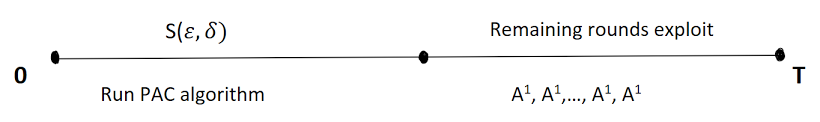
\includegraphics[height=30mm,width=180mm]{PAC.png}
	\label{fig:synth}
\end{figure}

Let $R_T$ be the total regret until time T. 
\begin{eqnarray}
R_T = S(\epsilon, \delta )  + \epsilon (T - S(\epsilon, \delta ) ) (1 - \delta) + \delta (T - S(\epsilon, \delta ) )
\end{eqnarray}

If $S(\epsilon, \delta ) = \frac{k \log(\frac{1}{\delta})}{\epsilon^2}$ and $ \delta = \frac{1}{T}$, then 
\begin{eqnarray}
 \nonumber R_T &=& S(\epsilon, \delta )  + \epsilon (T - S(\epsilon, \delta ) ) (1 - \delta) + \delta (T - S(\epsilon, \delta ) ) \\
   \nonumber &\leq & \frac{k \log(\frac{1}{\delta})}{\epsilon^2} + (1-\delta)\epsilon T + \delta T \\  
 &=&\frac{k \log(T)}{\epsilon^2} + \epsilon T + 1 
\end{eqnarray}

by tuning $\epsilon$ we get total regret of the order  $O(T^{2/3})$. 


\bibliography{stats710}
\end{document}


